\chapter{URG of the SIAM and its Spin and Charge Generalisations}\label{siamurg}
\section{The single-impurity Anderson model}
The model is the usual single-impurity Anderson model Hamiltonian.
\begin{equation}\begin{aligned}
	\label{andham}
	\mathcal{H} = \sum_{k\sigma}\epsilon_k \hat n_{k\sigma} + \sum_{k\sigma} \left(V_{k} c^\dagger_{k\sigma} c_{d\sigma} + h.c.\right) + \epsilon_{d}\sum_\sigma  \hat n_{d\sigma} +  U \hat n_{d\uparrow} \hat n_{d\downarrow}
\end{aligned}\end{equation}
To allow the calculation of both particle and hole kinetic energies, we will write the kinetic energy part as \(\sum_{k\sigma}\epsilon_k \tau_{k\sigma}\), where \(\tau = \hat n - \frac{1}{2}\) and drop the extra constant part.
\begin{equation}
	\label{model:siam}
	\mathcal{H} = \sum_{k\sigma}\epsilon_k \tau_{k\sigma} + \sum_{k\sigma} \left(V_{k} c^\dagger_{k\sigma} c_{d\sigma} + h.c.\right) + \epsilon_{d}\sum_\sigma  \hat n_{d\sigma} +  U \hat n_{d\uparrow} \hat n_{d\downarrow}
\end{equation}
\section{Calculation of renormalisation}
The renormalisation is
\begin{equation}\begin{aligned}
\label{newh}
c^\dagger_{q\beta}T \frac{1}{\omega - H^D}T^\dagger c_{q\beta} + T^\dagger c_{q\beta}\frac{1}{\omega^\prime - H^D}c^\dagger_{q\beta}T
\end{aligned}\end{equation}
We will be decoupling an electron \(q\beta\) at the energy shell \(\epsilon_q = \pm D\). The diagonal part (that comes down in the denominator) is
\begin{equation}\begin{aligned}
	\label{term1}
H^D = \epsilon_q \tau_{q\beta} + \epsilon_{d}\hat n_{d\beta} +  U \hat n_{d\beta} \hat n_{d\bar\beta}
\end{aligned}\end{equation}
The off-diagonal part is
\begin{equation}\begin{aligned}
	c^\dagger_{q\beta}T = V_q c^\dagger_{q\beta}c_{d\beta}
\end{aligned}\end{equation}

The renormalisation from a single electron \(q\beta\) is
\begin{equation}\begin{aligned}
	\Delta H &= c^\dagger_{q\beta}c_{d\beta} \frac{1|V_q|^2}{\omega - H^D}c_{d\beta}^\dagger c_{q\beta} + c_{d\beta}^\dagger c_{q\beta}\frac{1|V_q|^2}{\omega^\prime - H^D}c^\dagger_{q\beta}c_{d\beta} \\
		 &= c^\dagger_{q\beta}c_{d\beta} \frac{|V_q|^2}{\omega - D/2 - \epsilon_d - U \hat n_{d\bar\beta}}c_{d\beta}^\dagger c_{q\beta} + c_{d\beta}^\dagger c_{q\beta}\frac{|V_q|^2}{\omega^\prime - D/2}c^\dagger_{q\beta}c_{d\beta}\\
		 &=  \frac{\hat n_{q\beta}\left( 1 - \hat n_{d\beta} \right) |V_q|^2}{\omega - D/2 - \epsilon_d - U \hat n_{d\bar\beta}} + \frac{\hat n_{d\beta}\left( 1 - \hat n_{q\beta} \right) |V_q|^2}{\omega^\prime - D/2}
\end{aligned}\end{equation}

For comparing the two \(\omega\)s, we will use the relation eq.~\ref{omegarel}: \(\omega_0^1 + \omega^1_0 = H^D_0 + H^D_1\) where \(\omega_0^1 = \omega^\prime\). \(\omega^1_0\) however is not \(\omega\). This is because the relation assumes the \(\omega\)s to be calculated at the same energy - while \(\omega^\prime\) is calculated at energy \(-D\), \(\omega\) is at energy \(D\). The \(\omega_0^1\) should hence be the \(\omega\) at energy \(-D\), which is \(-\omega\). With this in mind, the relation says
\begin{equation}\begin{aligned}
	\omega^\prime - \omega = D/2 + \epsilon_d + U \hat n_{d\beta} - D/2 
\end{aligned}\end{equation}
This gives an expression of \(\omega^\prime\) in terms of \(\omega\). Substituting this into \(\Delta H\)  gives
\begin{equation}\begin{aligned}
	\Delta H &=  \frac{\hat n_{q\beta}\left( 1 - \hat n_{d\beta} \right) |V_q|^2}{\omega - D/2 - \epsilon_d - U \hat n_{d\bar\beta}} + \frac{\hat n_{d\beta}\left( 1 - \hat n_{q\beta}\right)|V_q|^2}{\omega - D/2 +\epsilon_d + U \hat n_{d\bar\beta}}
\end{aligned}\end{equation}
The total renormalisation from the entire shell \(\pm D\) is
\begin{equation}\begin{aligned}
	\label{vanilla:siam:ren}
	\Delta H &=  \sum_{q\beta}|V_q|^2\left[\frac{\hat n_{q\beta}\left( 1 - \hat n_{d\beta} \right) }{\omega - D/2 - \epsilon_d - U \hat n_{d\bar\beta}} + \frac{\hat n_{d\beta}\left( 1 - \hat n_{q\beta}\right)}{\omega - D/2 +\epsilon_d + U \hat n_{d\bar\beta}}\right] \\
		 &= \sum_q |V_q|^2 \left[\frac{\left(1 - \hat n_{d\beta}\right)\hat n_{d\overline\beta}}{\omega - \frac{1}{2}\epsilon_q - \epsilon_d - U} + \frac{\left(1 - \hat n_{d\beta}\right)\left( 1-\hat n_{d\overline\beta} \right)}{\omega - \frac{1}{2}\epsilon_q - \epsilon_d} + \frac{\hat n_{d\beta} \hat n_{d\overline\beta}}{\omega - \frac{1}{2}\epsilon_q + \epsilon_d + U} + \frac{\hat n_{d\beta}\left( 1- \hat n_{d\overline\beta}\right) }{\omega - \frac{1}{2}\epsilon_q + \epsilon_d}\right]
\end{aligned}\end{equation}
\section{Scaling equations for the SIAM}
Once we have the renormalisation for decoupling one electronic or hole state, we can just sum over the spins and momenta to get the total renormalisation upon decoupling the entire shells \(\pm \epsilon_q\). From the structure of \(\Delta \mathcal{H}\) in eq.~\ref{vanilla:siam:ren}, we can see that there are renormalisations to all three configuration energies of the impurity: the doublon energy \(E_2\) corresponding to the state  \(\hat n_{d\beta}\hat n_{d\overline\beta}\), the single energy \(E_1\) corresponding to (\(\hat n_{d\beta}(1 - \hat n_{d\overline\beta}) + \hat n_{d\overline\beta}(1 - \hat n_{d\beta})\), and the holon energy \(E_0\) corresponding to \((1 - \hat n_{d\beta})(1 - \hat n_{d\overline\beta}) + \hat n_{d\overline\beta}(1 - \hat n_{d\beta})\).
\begin{equation}\begin{aligned}
	\label{urg-siam}
	\Delta E_2 &= +2\sum_{q}\frac{|V_q|^2}{\omega - \frac{1}{2}\epsilon_q + \epsilon_d + U }\\
	\Delta E_1 &= +\sum_{q}\frac{|V_q|^2}{\omega - \frac{1}{2}\epsilon_q + \epsilon_d} + \sum_{q}\frac{|V_q|^2}{\omega - \frac{1}{2}\epsilon_q - \epsilon_d - U}\\
	\Delta E_0 &= +2\sum_{q}\frac{|V_q|^2}{\omega - \frac{1}{2}\epsilon_q - \epsilon_d}
\end{aligned}\end{equation}
Using the relations \(\epsilon_d = E_1 - E_0\) and \(U = E_2 + E_0 - 2E_1\), we can write
\begin{equation}\begin{aligned}
	\Delta \epsilon_d &= +\sum_{q}\frac{|V_q|^2}{\omega - \frac{1}{2}\epsilon_q + \epsilon_d} + \sum_{q}\frac{|V_q|^2}{\omega - \frac{1}{2}\epsilon_q - \epsilon_d - U} - 2\sum_{q}\frac{|V_q|^2}{\omega - \frac{1}{2}\epsilon_q - \epsilon_d}\\
	\Delta U &= \sum_{q}\frac{2|V_q|^2}{\omega - \frac{1}{2}\epsilon_q + \epsilon_d + U } + \sum_{q}\frac{2|V_q|^2}{\omega - \frac{1}{2}\epsilon_q - \epsilon_d} - \sum_{q}\frac{2|V_q|^2}{\omega - \frac{1}{2}\epsilon_q + \epsilon_d} - \sum_{q}\frac{2|V_q|^2}{\omega - \frac{1}{2}\epsilon_q - \epsilon_d - U}\\
\end{aligned}\end{equation}
\section{Connection to poor man's scaling}\label{urg2pms}
To obtain the results of Poor Man's scaling \cite{haldane}\cite{Jefferson},  we can look at various regimes. First we look at the case when both \(\epsilon_d\) and \(U\) are small such that both the singly-occupied and doubly-occupied subspaces of the impurity are comfortably inside the bandwidth, \(U,\epsilon_d \ll \epsilon_q\). We can then ignore the \(\epsilon_d\) and \(U\) in the denominator compared to the \(\epsilon_q\).
\begin{equation}\begin{aligned}
\Delta \epsilon_d &= \sum_{q}\frac{|V_q|^2}{\omega - \frac{1}{2}\epsilon_q} + \sum_{q}\frac{|V_q|^2}{\omega - \frac{1}{2}\epsilon_q} - 2\sum_{q}\frac{|V_q|^2}{\omega - \frac{1}{2}\epsilon_q}\\
\Delta U &= 2\sum_{q}\frac{|V_q|^2}{\omega - \frac{1}{2}\epsilon_q} + 2\sum_{q}\frac{|V_q|^2}{\omega - \frac{1}{2}\epsilon_q} - 2\sum_{q}\frac{|V_q|^2}{\omega - \frac{1}{2}\epsilon_q} - 2\sum_{q}\frac{|V_q|^2}{\omega - \frac{1}{2}\epsilon_q}
\end{aligned}\end{equation}
Assuming the upper and lower band edges are symmetrical such that \(\sum_{-D} = \sum_D\), we get \(\Delta \epsilon_d = \Delta U = 0\). 

In the regime \(U \gg \epsilon_q \gg \epsilon_d\), the doubly-occupied state is far above the bandwidth. We can now ignore the terms that have \(U\) in the denominator. We get
\begin{equation}\begin{aligned}
\Delta \epsilon_d &= \sum_{q}\frac{|V_q|^2}{\omega - \frac{1}{2}\epsilon_q} - 2\sum_{q}\frac{|V_q|^2}{\omega - \frac{1}{2}\epsilon_q}\\
\Delta U &= 2\sum_{q}\frac{|V_q|^2}{\omega - \frac{1}{2}\epsilon_q}  - 2\sum_{q}\frac{|V_q|^2}{\omega - \frac{1}{2}\epsilon_q} 
\end{aligned}\end{equation}
Again assuming symmetrical upper and lower edges, and isotropic dispersion \(\epsilon_q=D\) and \(\sum_q |V|^2 = \frac{\Delta}{\pi}|\delta D|\), we get
\begin{equation}\begin{aligned}
\Delta U &= 0\\
\delta \epsilon_d &= -\frac{\Delta}{\pi}\frac{1}{\omega - \frac{1}{2} D}
\end{aligned}\end{equation}
There we replaced the difference symbol \(\Delta\) with \(\delta\) to avoid confusion with the hybridisation \(\Delta \sim \sum V^2\). For low quantum fluctuations, we can ignore the renormalisation in the couplings and replace \(\omega\) with the initial conduction electron energy: \(\omega = \epsilon_q\tau_{q\beta} = -\frac{1}{2} D\).
\begin{equation}\begin{aligned}
\delta \epsilon_d &= \frac{\Delta}{\pi}\frac{\delta D}{D}
\end{aligned}\end{equation}
This is the one-loop scaling equation.
\section{Preservation of particle-hole symmetry}
The Anderson model Hamiltonian, eq.~\ref{andham}, has an impurity particle-hole symmetry for a certain condition of the couplings. To see this, we apply the particle-hole transformation \(c_k \to c^\dagger_k, c_d \to -c^\dagger_d\) to the Hamiltonian. Since we are looking at the impurity symmetry, we will only look at the terms involving the impurity. The particle-hole symmetry of the conduction bath is a separate thing and that requires a specific lattice. Hence we will not consider kinetic energy term in this discussion. The rest of the terms transform as
\begin{gather}
    \epsilon_d \sum_\sigma \hat n_{d\sigma} \to 2\epsilon_d - \epsilon_d \sum_\sigma \hat n_{d\sigma}\label{imp1}\\
U \hat n_{d\uparrow}\hat n_{d\downarrow} \to U \hat n_{d\uparrow}\hat n_{d\downarrow} - U\sum_\sigma \hat n_{d\sigma} + U\label{imp2}\\
\sum_{k\sigma}V(k)c^\dagger_{k\sigma}c_{d\sigma} + hc \to \sum_{k\sigma}-V(k)c_{k\sigma}c^\dagger_{d\sigma} + hc = \sum_{k\sigma}V^*(k)c^\dagger_{k\sigma}c_{d\sigma} + hc \label{hop}
\end{gather}
The impurity-bath hopping term can be made symmetric by making \(V(k)\) real; we would then have, from eq.~\ref{hop},
\begin{equation}\begin{aligned}
	V(k)\left(c^\dagger_{k\sigma}c_{d\sigma} + c^\dagger_{d\sigma}c_{k\sigma}\right)\to V(k)\left(c^\dagger_{d\sigma}c_{k\sigma} + c^\dagger_{k\sigma}c_{d\sigma}\right)
\end{aligned}\end{equation}
The impurity diagonal terms, \(\epsilon_d\) and \(U\), require a specific condition. Combining eqs.~\ref{imp1} and \ref{imp2},
\begin{equation}\begin{aligned}
	\epsilon_d\hat n_{d\sigma} + U\hat n_{d\uparrow}\hat n_{d\downarrow} \to \left(-\epsilon_d - U\right)\hat n_{d\sigma} + U\hat n_{d\uparrow}\hat n_{d\downarrow}
\end{aligned}\end{equation}
We dropped some constant terms in the transformed Hamiltonian. For particle-hole symmetry, the left and right hand sides must be same. The required condition is thus 
\begin{equation}\begin{aligned}
	\label{phs}
\epsilon_d = -\epsilon_d - U \implies \epsilon_d + \frac{1}{2} U = 0
\end{aligned}\end{equation}
\begin{minipage}{0.5\textwidth}
    This same condition can be obtained in a more physical way. If we consider the singly-occupied state of the impurity as the reference state, the doubly-occupied state is the particle-excitation and the vacant state is the hole excitation. The energy of this particle state is \(E_2 = 2\epsilon_d + U\) and that of the hole state is \(E_0 = 0\). Particle-hole symmetry then requires the particle and hole levels to be degenerate, which means \(E_2 = E_0\), and we recover the condition eq.~\ref{phs}.
\end{minipage}
\hfill
\begin{minipage}{0.4\textwidth}
    \centering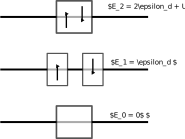
\includegraphics[width=0.8\textwidth]{phsymm.pdf}
    \captionof{figure}{Particle and hole excitations of the impurity}
\end{minipage}

Since the URG is unitary, if we start from a model that is particle-hole symmetric, the RG equations should uphold that symmetry. What this means is that if we have \(\epsilon_d + \frac{1}{2} U = 0\) in the bare model, the new couplings should also satisfy \(\epsilon_d^\prime + \frac{1}{2} U^\prime = 0\). This means we must have 
\begin{equation}\begin{aligned}
	\Delta\left(\epsilon_d + \frac{1}{2} U\right) = 0
\end{aligned}\end{equation}
The quantity \(\gamma = \epsilon_d + \frac{1}{2} U\) is thus an RG-invariant for the particle-hole symmetric model; it does not change under the RG flow. It is often referred to as the asymmetry parameter; it quantifies the asymmetry in the model. We need to check if our equations satisfy this. Looking at the RG equations for \(\epsilon_d\) and \(U\), we can find the RG equation for the asymmetry parameter. The slightly easier way is to just note that the renormalisation in \(E_2\) should be equal to the renormalisation in \(E_0\), in order for p-h symmetry to hold.
\begin{equation}\begin{aligned}
\Delta E_2 &= 2 \frac{\Delta}{\pi}\frac{1}{\omega - D + \epsilon_d + U}, \Delta E_0 &= 2 \frac{\Delta}{\pi}\frac{1}{\omega - D - \epsilon_d}
\end{aligned}\end{equation}
If we start with a particle-hole symmetric model, we will have \(-\epsilon_d = \epsilon_d + U\). Substituting that gives \(\Delta E_2= \Delta E_0\). This shows that the doublon and holon states remain equidistant from the single-particle level, thus maintaining particle-hole symmetry along the flow.
\section{Numerical analysis of the particle-hole symmetric RG equations}
We will specialize to the particle-hole symmetric case, \(2\epsilon_d + U = 0\), and a symmetric energy shell \(\epsilon_q = D\), and look at the scaling behavior of \(\epsilon_d\).
\begin{equation}\begin{aligned}
	\Delta \epsilon_d = -4|V|^2 \frac{\epsilon_d}{\left( \omega - \frac{1}{2}D \right)^2 - \epsilon_d^2}
\end{aligned}\end{equation}
Since the equation is symmetric under \(\epsilon_d \to -\epsilon_d\), we might as well work with the magnitude of the onsite energy:
\begin{equation}\begin{aligned}
	\Delta |\epsilon_d| = -4|V|^2 \frac{|\epsilon_d|}{\left( \omega - \frac{1}{2}D \right)^2 - \epsilon_d^2}
\end{aligned}\end{equation}
Depending on the signature of the denominator, the flows will be either relevant or irrelevant.
\begin{figure}[!htpb]
	\centering
	\includegraphics[width=0.99\textwidth]{../figures/ed_pure_siam.pdf}
	\caption{Left: Irrelevant flow towards \(|\epsilon_d|=0\), at low \(\omega\). Right: Relevant flow towards large \(|\epsilon_d|\), at large \(\omega\). The former can be thought of as the projection of the strong-coupling flow on to the \(\epsilon_d-D\) plane. The latter is the flow towards the local moment fixed point, if we start from a negative \(\epsilon_d\).}
\end{figure}
For the flow to the local moment fixed point, the fixed point value of \(|\epsilon_d|\) grows as we increase the bandwidth. This implies that for a thermodynamically large system, the local moment fixed point will be at \(-\epsilon_d \to \infty\). This behavior is shown in fig.~\ref{edvsD}.
\begin{figure}[htpb]
	\centering
	\includegraphics[width=0.6\textwidth]{../figures/ed_vs_size.pdf}
	\caption{Change in fixed point value of \(|\epsilon_d|\) with system size.}
	\label{edvsD}
\end{figure}
\section{Introduction of spin-exchange and charge isospin-exchange interactions into the SIAM: the generalised SIAM}
We will now study the generalised SIAM obtained by introducing spin-exchange and charge isospin-exchange interactions between the impurity and the conduction bath. Such terms are generated when one does a Schrieffer-Wolff transformation on the SIAM, but we will find it prudent to keep these terms in the bare model itself.

The spin-exchange interaction has the form
\begin{equation}\begin{aligned}
	J \vec{S_d}\cdot\vec{s} = J \left[S_d^z s^z + \frac{1}{2}\left( S_d^+ s^- + S_d^- s^+ \right) \right] ~,
\end{aligned}\end{equation}
where \(\vec S_d = \left(S_d^x, S_d^y, S_d^z\right) = \sum_{\alpha\beta}\vec \sigma_{\alpha\beta}c^\dagger_{d\alpha}c_{d\beta}\) is the impurity spin operator, \(\vec s = \sum_{kk^\prime\alpha\beta}\vec \sigma_{\alpha\beta}c^\dagger_{k\alpha}c_{k^\prime\beta}\) is the spin operator for the conduction bath and \(J\) is the spin-exchange coupling. The bath spin operator actually acts locally, as can be seen by Fourier transforming to real space (using the definition \(f(k) = \frac{1}{\sqrt N}\sum_r g(r)\exp(ikr)\)):
\begin{equation}\begin{aligned}
	\vec s = \sum_{k k^\prime r r^\prime} \frac{1}{N} e^{ikr - ik^\prime r^\prime} \vec \sigma_{\alpha\beta} c^\dagger_{r\alpha} c_{r^\prime\beta} = \sum_{rr^\prime}\frac{1}{N}\vec \sigma_{\alpha\beta} c^\dagger_{r\alpha} c_{r^\prime\beta} N \delta(r)\delta(r^\prime) = \vec \sigma_{\alpha\beta} c^\dagger_{0\alpha} c_{0\beta}
\end{aligned}\end{equation}

In order to introduce the charge isospin coupling, we define the Nambu spinor \cite{nambu,anderson_superc} \(\psi^k = \left( c_{k\uparrow} \quad c^\dagger_{k\downarrow} \right)\), and the charge isospin \cite{charge-kondo-Zitko} for the mobile conduction electrons
\begin{equation}\begin{aligned}
\vec C = \sum_{kk^\prime} {\psi^k}^\dagger \vec S \psi^{k^\prime} = \frac{1}{2}\sum_{kk^\prime\alpha\beta} {\psi^k_\alpha}^\dagger \vec \sigma_{\alpha\beta} \psi^{k^\prime}_\beta
\end{aligned}\end{equation}
The various components of the isospin are
\begin{equation}\begin{aligned}
	C^z &= \sum_{kk^\prime\sigma}\frac{1}{2} {\psi^k_\sigma}^\dagger \sigma^z_{\sigma\sigma} \psi^{k^\prime}_\sigma = \frac{1}{2}\sum_{kk^\prime\sigma}\left(c^\dagger_{k\sigma}c_{k^\prime \sigma} - \frac{1}{2}\delta_{kk^\prime}\right)\label{diagonalCz}\\
	C^x &= \sum_{kk^\prime\sigma}\frac{1}{2} {\psi^k_\sigma}^\dagger \sigma^x_{\sigma\overline\sigma} \psi^{k^\prime}_{\overline\sigma} = \sum_{kk^\prime\sigma} \frac{\sigma}{4}\left( c^\dagger_{k\sigma}c^\dagger_{k^\prime\overline\sigma} + \text{h.c.} \right) \\
	C^y &= \sum_{kk^\prime\sigma}\frac{1}{2} {\psi^k_\sigma}^\dagger \sigma^y_{\sigma\overline\sigma} \psi^{k^\prime}_{\overline\sigma} = \sum_{kk^\prime\sigma} - \frac{i\sigma}{4}\left( c^\dagger_{k\sigma}c^\dagger_{k^\prime\overline\sigma} - \text{h.c.} \right)\\
\end{aligned}\end{equation}
It is easy to verify that these operators satisfy the SU(2) commutation algebra. For example, if we write \(C^x = A + A^\dagger\) and \(C^y = B + B^\dagger\), then \(\left[ C^x, C^y \right] = \left[ A, B^\dagger \right] - \text{h.c.}\), where
\begin{equation}\begin{aligned}
	\left[ A, B^\dagger \right] = \frac{1}{4}\sum_{kk^\prime,qq^\prime}\left[ c^\dagger_{k\uparrow}c^\dagger_{k^\prime \downarrow}, i c_{q^\prime \downarrow}c_{q \uparrow} \right] = \frac{i}{4}\sum_{kq}\left(c^\dagger_{k\uparrow}c_{q \uparrow} - c_{k \downarrow}c^\dagger_{q \downarrow}\right)
\end{aligned}\end{equation}
and therefore
\begin{equation}\begin{aligned}
	\implies \left[ C^x, C^y \right] = \frac{i}{2}\sum_{kq}\left(c^\dagger_{k\uparrow}c_{q \uparrow} - c_{k \downarrow}c^\dagger_{q \downarrow}\right) = i C^z
\end{aligned}\end{equation}
There are similar operators for the impurity electron:
\begin{equation}\begin{aligned}
	\psi_d = \left( c_{d\uparrow} \quad c^\dagger_{d\downarrow}\right), &&\vec C_d = \frac{1}{2}\sum_{\beta} {\psi_{d,\alpha}}^\dagger \vec \sigma_{\alpha\beta} \psi_{d,\beta}
\end{aligned}\end{equation}
The full charge-Kondo interaction can now be written down in terms of these isospins:
\begin{equation}\begin{aligned}
	K \vec{C_d}\cdot\vec{C} = K \left[C_d^z C^z + \frac{1}{2}\left(C_d^+ C^-+ C_d^- C^+\right)\right]
\end{aligned}\end{equation}
where \(C^\pm \equiv C^x \pm iC^y\).
\begin{equation}\begin{aligned}
	C^+ = \sum_{kk^\prime} c^\dagger_{k\uparrow}c^\dagger_{k^\prime\downarrow}, && C^- = \sum_{kk^\prime}c_{k^\prime\downarrow}c_{k\uparrow}
\end{aligned}\end{equation}
The full generalised Anderson model Hamiltonian, at particle-hole symmetry, is
\begin{equation}\begin{aligned}
	\mathcal{H} = \sum_{k\sigma}\epsilon_k \tau_{k\sigma} + \epsilon_d \left( \hat n_{d \uparrow} - \hat n_{d \downarrow} \right) ^2 + \sum_{k\sigma} \left(V_{k} c^\dagger_{k\sigma} c_{d\sigma} + h.c.\right) +J \vec{S_d}\cdot\vec{s} + K \vec{C_d}\cdot\vec{C}
\end{aligned}\end{equation}

For the URG analysis, at each RG step, we decouple the electronic states \(q\beta\) on the \(k-\)space shell of radius\(\Lambda_j\). For simplicity, we will only consider those diagonal terms in the denominator that either have both \(q\beta\) and \(q\overline\beta\) or  both \(q\beta\) and \(d\) or both \(q\overline\beta\) and \(d\). Terms that have purely \(q\overline\beta\) will not be considered. Also, the scattering between just \(d\) and \(q\overline\beta\) can be ignored since it is diagonal in \(q\beta\). 
The diagonal (number-preserving) part is
\begin{equation}\begin{aligned}
	H_D = \sum_\beta\epsilon_q\tau_{q\beta} + \epsilon_d \left( \hat n_{d \uparrow} - \hat n_{d \downarrow} \right) ^2 + J S^z_ds^z_{q} + K C^z_d C^z_q\\
\end{aligned}\end{equation}
where \(s_q^z = \frac{1}{2}\left(\hat n_{q\uparrow} - \hat n_{q\downarrow}\right)\) and \(C_q^z = \frac{1}{2}\left(\hat n_{q \uparrow} + \hat n_{q \downarrow} - 1\right)\). The off-diagonal part is:
\begin{equation}\begin{aligned}
	H_X = \sum_{\beta=\uparrow,\downarrow}\left[V c^\dagger_{q\beta}c_{d\beta} + \frac{1}{2}J \sum_{k<\Lambda_N}\left\{\left(\hat n_{d \beta} - \hat n_{d \overline\beta}\right) \frac{1}{2} c^\dagger_{k\beta}c_{q\beta} + c^\dagger_{d\beta}c_{d\overline\beta}c^\dagger_{k\overline\beta}c_{q \beta}\right\} + \frac{1}{2}K \sum_{k<\Lambda_N}\left\{\left(\hat n_d -1\right)\frac{1}{2}c^\dagger_{k\beta}c_{q\beta} + \right.\right.\\
\left.\left.c^\dagger_{d\beta}c^\dagger_{d\overline\beta}c_{k\overline\beta}c_{q\beta}\right\}\right] + \text{h.c.}~.
\end{aligned}\end{equation}

\section{Calculation of renormalisation}
\subsection{Renormalisation of the impurity energy \(\epsilon_d\)}
The coupling \(\epsilon_d\) is renormalised by three kinds of vertices: \(V^2\), \(J^2\) and \(K^2\). We now consider these processes in order. We define \(\sum_q \hat n_{q\beta} = \sum_q \left( 1 - \hat n_{q\beta} \right) \equiv n_j\) as the number of states being decoupled in either the particle or the hole sectors at the \(j^\text{th}\) RG step.

The renormalisation arising from the first kind of terms, in the particle sector, is
\begin{equation}\begin{aligned}
	\sum_{q\beta}c^\dagger_{q\beta}c_{d\beta}\frac{V^2}{\omega - H_D}c^\dagger_{d\beta}c_{q\beta} = \sum_{q\beta}V^2 \hat n_{q\beta} \left( 1 - \hat n_{d\beta} \right)\left( \frac{1-\hat n_{d \overline\beta }}{\omega - E_0} + \frac{\hat n_{d \overline\beta}}{\omega^\prime - E_1}\right) = V^2 n_j\sum_{\beta}\left( 1 - \hat n_{d\beta} \right)\left( \frac{1-\hat n_{d \overline\beta }}{\omega - E_0} + \frac{\hat n_{d \overline\beta}}{\omega^\prime - E_1}\right)
\end{aligned}\end{equation}
\(q\) runs over the momentum states that are being decoupled at this RG step: \(|q| = \Lambda_j\). \(E_{1,0}\) are the diagonal parts of the Hamiltonian at \(\hat n_{d\overline \beta}=0,1\) respectively. The kinetic energy of the diagonal part is always \(\frac{D}{2}\), because we are either exciting the ground state at energy \(-\frac{D}{2}\) to an excited state at energy \(\frac{D}{2}\). Also, \(\hat n_{d\beta}=1\) because of the \(c^\dagger_{d\beta}\) in front of the Greens function. We assume here that we scatter starting from a state in which \(s_q^z = C_q^z = 0\). That is, \(\left<\hat n_{q \uparrow}\right> = \left<\hat n_{q \downarrow}\right> = \frac{1}{2}\). Applying \(c_{q\beta}\) on such a state leaves us with \(C^z = - \frac{1}{2}\) and \(s^z_q = \frac{1}{2}\overline\beta\). We also know that
\begin{equation}\begin{aligned}
	\hat n_{d\beta}=1,
	\begin{cases}
		\hat n_{d\overline\beta}=0 &\implies S_d^z = \frac{1}{2}\beta, C_d^z = 0, \epsilon_d\left(\hat n_{d\uparrow} - \hat n_{d \downarrow}\right)^2 = \epsilon_d\\	
		\hat n_{d\overline\beta}=1 &\implies S_d^z = 0, C_d^z = \frac{1}{2}, \epsilon_d\left(\hat n_{d\uparrow} - \hat n_{d \downarrow}\right)^2 = 0
	\end{cases}
\end{aligned}\end{equation}
Combining all this, we can write \(E_1 = \frac{D}{2} - \frac{K}{4}\) and \(E_0 = \frac{D}{2} + \epsilon_d - \frac{J}{4}\). In order to relate \(\omega\) with \(\omega^\prime\), we will replace these quantum fluctuation scales by the current renormalised values of the diagonal part of the initial state from which we started scattering:
\begin{equation}\begin{aligned}
	\omega = -\frac{D}{2}, \omega^\prime = -\frac{D}{2} + \epsilon_d \implies \omega^\prime = \omega + \epsilon_d
\end{aligned}\end{equation}
Substituting the values of \(E_{0,1}\) and \(\omega^\prime\), we get
\begin{equation}\begin{aligned}
	\label{ren_ed_Vp}
	V^2 n_j\sum_{\beta}\left( 1 - \hat n_{d\beta} \right)\left( \frac{1-\hat n_{d \overline\beta }}{\omega - \frac{D}{2} - \epsilon_d + \frac{J}{4}} + \frac{\hat n_{d \overline\beta}}{\omega - \frac{D}{2} + \epsilon_d + \frac{K}{4}}\right)
\end{aligned}\end{equation}

Performing a similar calculation for the hole sector gives the contribution:
\begin{equation}\begin{aligned}
	\label{ren_ed_Vh}
	V^2 n_j\sum_{\beta}\hat n_{d\beta}\left( \frac{1-\hat n_{d \overline\beta }}{\omega - \frac{D}{2} + \epsilon_d + \frac{K}{4}} + \frac{\hat n_{d \overline\beta}}{\omega - \frac{D}{2} - \epsilon_d + \frac{J}{4}}\right)
\end{aligned}\end{equation}

We now come to the second type of terms: spin-spin. We first look at the particle sector:
\begin{equation}\begin{aligned}
	\label{ren_ed_Jpp}
	\frac{J^2}{4}\sum_{q\beta}c^\dagger_{d\overline\beta}c_{d\beta}c^\dagger_{q\beta}c_{q\overline\beta} \frac{1}{\omega - H_D}c^\dagger_{d\beta}c_{d\overline\beta}c^\dagger_{q\overline\beta}c_{q\beta} = \frac{J^2}{4} n_j\frac{1}{\omega - \frac{D}{2} + \frac{J}{4}} \sum_{\beta}\hat n_{d\overline\beta}\left( 1 - \hat n_{d\beta} \right)
\end{aligned}\end{equation}
The diagonal part in the denominator was simple to deduce in this case, because the nature of the scattering requires the spins \(S_d^z\) and \(s_q^z\) to be anti-parallel. In the hole sector, we have
\begin{equation}\begin{aligned}
	\label{ren_ed_Jph}
	\frac{J^2}{4} n_j\frac{1}{\omega - \frac{D}{2} + \frac{J}{4}} \sum_{\beta}\hat n_{d\beta}\left( 1 - \hat n_{d\overline\beta} \right)
\end{aligned}\end{equation}

The final kind of scattering is the \(K^2\) type. Similar to the \(J^2\) term, we get the following contribution:. 
\begin{equation}\begin{aligned}
	\label{ren_ed_Kpp}
	\frac{K^2}{4}\sum_{q\beta}c^\dagger_{q\beta}c^\dagger_{q\overline\beta}c_{d\overline\beta}c_{d\beta} \frac{1}{\omega - H_D}c^\dagger_{d\beta}c^\dagger_{d\overline\beta}c_{q\overline\beta}c_{q\beta} = \frac{K^2}{2} n_j\frac{1}{\omega - \frac{D}{2} + \frac{K}{4}} \left(1 - \hat n_{d \uparrow}\right) \left( 1 - \hat n_{d \downarrow} \right)
\end{aligned}\end{equation}
in the particle sector, and
\begin{equation}\begin{aligned}
	\label{ren_ed_Kph}
	\frac{K^2}{2} n_j\frac{1}{\omega - \frac{D}{2} + \frac{K}{4}} \hat n_{d\uparrow}\hat n_{d \downarrow}
\end{aligned}\end{equation}
in the hole sector.

We now have all possible renormalisation to the impurity energy \(\epsilon_d\). To actually compute the renormalisation, we will first calculate the renormalisation in the energies \(\epsilon_0, \epsilon_1\) and \(\epsilon_2\) of the impurity states \(\ket{\hat n_d = 0}, \ket{\hat n_d = 1}, \ket{\hat n_d = 2}\) respectively. The renormalisation of these states are given by the following terms:
\begin{itemize}
	\item \(\Delta \epsilon_0\) is given by the renormalisation of the term \(\left(1 - \hat n_{d\uparrow}\right)\left(1 - \hat n_{d \downarrow}\right)\)
	\item \(\Delta \epsilon_1\) is given by the renormalisation of either \(\left(1 - \hat n_{d\uparrow}\right)\hat n_{d \downarrow}\) or \(\left(1 - \hat n_{d\downarrow}\right)\hat n_{d \uparrow}\)
	\item \(\Delta \epsilon_2\) is given by the renormalisation of \(\hat n_{d\uparrow}\hat n_{d \downarrow}\)
\end{itemize}
From eqs.~\ref{ren_ed_Vp}, \ref{ren_ed_Vh}, \ref{ren_ed_Jpp}, \ref{ren_ed_Jph}, \ref{ren_ed_Kpp} and \ref{ren_ed_Kph}, we write
\begin{equation}\begin{aligned}
	\Delta \epsilon_0 = \Delta \epsilon_2 = \frac{2V^2 n_j}{\omega - \frac{D}{2} - \epsilon_d + \frac{J}{4}} + \frac{K^2 n_j/2}{\omega - \frac{D}{2} + \frac{K}{4}}, && \Delta \epsilon_1 = \frac{2V^2 n_j}{\omega - \frac{D}{2} + \epsilon_d + \frac{K}{4}} + \frac{J^2 n_j/2}{\omega - \frac{D}{2} + \frac{J}{4}}
\end{aligned}\end{equation}
We had started with a particle-hole symmetric Hamiltonian \((2\epsilon_d + U = 0)\); the fact that \(\Delta \epsilon_0 = \Delta \epsilon_2\) means the RG transformation has preserved that symmetry. The renormalisation of \(\epsilon_d\) is simply the renormalisation in the energy difference between the singly-occupied and vacant impurity levels: \(\Delta \epsilon_d = \Delta \epsilon_1 - \Delta \epsilon_0\). This gives our first RG equation:
\begin{equation}\begin{aligned}
	\Delta \epsilon_d = 2V^2 n_j\left(\frac{1}{\omega - \frac{D}{2} + \epsilon_d + \frac{K}{4}} - \frac{1}{\omega - \frac{D}{2} - \epsilon_d + \frac{J}{4}}\right) + \frac{n_j}{2}\left(\frac{J^2}{\omega - \frac{D}{2} + \frac{J}{4}} - \frac{K^2}{\omega - \frac{D}{2} + \frac{K}{4}}\right)
\end{aligned}\end{equation}

\subsection{Renormalisation of the hybridisation \(V\)}
Renormalisation of \(V\) happens through two kinds of processes: \(VJ\) and \(VK\). In order words, the two vertices involve one single-particle scattering and one spin or isospin exchange respectively. We first look at the vertices that involve a spin-exchange scattering.

Within spin-exchange, the scattering can be either via \(S_d^z\) or through \(S_d^\pm\). For the first kind, we have the following contribution in the particle sector:
\begin{equation}\begin{aligned}
	\sum_{q\beta} Vc^\dagger_{q\beta} c_{d\beta} \frac{1}{\omega - H_D}\frac{1}{4}J \sum_{k} \left(\hat n_{d\beta} - \hat n_{d\overline\beta}\right) c^\dagger_{k\beta}c_{q\beta} = \frac{1}{4}V J n_j \frac{1}{\omega^\prime - E} \sum_{k\beta} \left(1 - \hat n_{d\overline\beta}\right) c_{d\beta}c^\dagger_{k\beta}
\end{aligned}\end{equation}
Note that the \(c_{d\beta}\) in front of the Greens function resulted in \(\left(\hat n_{d\beta} - \hat n_{d\overline\beta}\right) \to \left(1 - \hat n_{d\overline\beta}\right)\). The intermediate state is characterised by \(\hat n_{d\beta} = 1 - \hat n_{d \overline \beta} = 1\), which means that \(E = \frac{D}{2} + \epsilon_d - \frac{J}{4}\). Moreover, \(\omega^\prime = -\frac{D}{2} + \epsilon_d = \omega + \epsilon_d\). Therefore, the renormalisation becomes
\begin{equation}\begin{aligned}
	-\frac{n_j}{4}V J \frac{1}{\omega - \frac{D}{2} + \frac{J}{4}} \sum_{k\beta}\left(1 - \hat n_{d\overline\beta}\right) c^\dagger_{k\beta} c_{d\beta}
\end{aligned}\end{equation}
One can generate another such process by exchanging the single-particle process and the spin-exchange process:
\begin{equation}\begin{aligned}
	\sum_{q\beta} \frac{1}{4}J \sum_{k} \left(\hat n_{d\beta} - \hat n_{d\overline\beta}\right) c^\dagger_{q\beta}c_{k\beta} \frac{1}{\omega - H_D} V c^\dagger_{d\beta} c_{q\beta}
\end{aligned}\end{equation}
This is simply the Hermitian conjugate of the previous contribution. Combining this with the previous then gives
\begin{equation}\begin{aligned}
	-\frac{n_j}{4}V J \frac{1}{\omega - \frac{D}{2} + \frac{J}{4}} \sum_{k\beta}\left(1 - \hat n_{d\overline\beta}\right)\left(c^\dagger_{d\beta} c_{k\beta} + \text{h.c.}\right)
\end{aligned}\end{equation}

We now consider the spin-exchange processes involving \(S_d^\pm\):
\begin{equation}\begin{aligned}
	\sum_{q\beta} Vc^\dagger_{q\beta} c_{d\beta} \frac{1}{\omega - H_D}\frac{1}{2}J \sum_{k} c^\dagger_{d\beta}c_{d\overline\beta} c^\dagger_{k\overline\beta}c_{q\beta} = \frac{1}{2}V J n_j \frac{1}{\omega^\prime - E} \sum_{k\beta} \left(1 - \hat n_{d\beta}\right) c_{d\overline\beta}c^\dagger_{k\overline\beta}
\end{aligned}\end{equation}
We again have \(E = \frac{D}{2} + \epsilon_d - \frac{J}{4}\) and \(\omega^\prime = \omega + \epsilon_d\), which gives
\begin{equation}\begin{aligned}
	-\frac{1}{2}V J n_j \frac{1}{\omega - \frac{D}{2} + \frac{J}{4}} \sum_{k\beta} \left(1 - \hat n_{d\beta}\right)c^\dagger_{k\overline\beta} c_{d\overline\beta}
\end{aligned}\end{equation}
Combining this with the Hermitian conjugate obtained from exchanging the processes gives
\begin{equation}\begin{aligned}
	-\frac{1}{2}V J n_j \frac{1}{\omega - \frac{D}{2} + \frac{J}{4}} \sum_{k\beta} \left(1 - \hat n_{d\beta}\right)\left(c^\dagger_{k\overline\beta} c_{d\overline\beta} + \text{h.c.}\right)
\end{aligned}\end{equation}

We now look at the hole sector. The first term gives
\begin{equation}\begin{aligned}
	\sum_{q\beta} V c^\dagger_{d\beta} c_{q\beta} \frac{1}{\omega - H_D}\frac{1}{4}J \sum_{k} \left(\hat n_{d\beta} - \hat n_{d\overline\beta}\right) c^\dagger_{q\beta}c_{k\beta} = -\frac{1}{4}V J n_j \frac{1}{\omega^\prime - E} \sum_{k\beta} \hat n_{d\overline\beta} c^\dagger_{d\beta}c_{k\beta}
\end{aligned}\end{equation}
Using identical arguments as above, we find \(E = \frac{D}{2} + \epsilon_d - \frac{J}{4}\) and \(\omega^\prime = \omega + \epsilon_d\), so the hole contribution becomes
\begin{equation}\begin{aligned}
	-\frac{n_j}{4}V J \frac{1}{\omega - \frac{D}{2} + \frac{J}{4}} \sum_{k\beta}\hat n_{d\overline\beta} c^\dagger_{d\beta} c_{k\beta}
\end{aligned}\end{equation}
The other hole contributions can be similarly obtained; the total renormalisation to \(V\) from \(VJ\) processes are
\begin{equation}\begin{aligned}
	-\frac{3n_j}{4}V J \frac{1}{\omega - \frac{D}{2} + \frac{J}{4}} \sum_{k\beta}\left(c^\dagger_{d\beta} c_{k\beta} + \text{h.c.}\right)
\end{aligned}\end{equation}

We now look at the \(VK\) processes. The first one is
\begin{equation}\begin{aligned}
	\sum_{q\beta} Vc^\dagger_{q\beta} c_{d\beta} \frac{1}{\omega - H_D}\frac{1}{4}K \sum_{k} \left(\hat n_{d} - 1\right) c^\dagger_{k\beta}c_{q\beta} = -\frac{1}{4}V K n_j \frac{1}{\omega - \frac{D}{2} + \frac{K}{4}}  \hat n_d\sum_{k\beta} c^\dagger_{k\beta}c_{d\beta}
\end{aligned}\end{equation}
The exchanged process again gives the Hermitian conjugate, so the combined contribution is
\begin{equation}\begin{aligned}
	-\frac{1}{4}V K n_j \frac{1}{\omega - \frac{D}{2} + \frac{K}{4}}  \hat n_d\sum_{k\beta} \left(c^\dagger_{k\beta}c_{d\beta} + \text{h.c.}\right)
\end{aligned}\end{equation}

The isospin-flip vertex gives
\begin{equation}\begin{aligned}
	\sum_{q\beta} V c^\dagger_{q\beta} c_{d\beta} \frac{1}{\omega - H_D}\frac{1}{2}K \sum_{k} c^\dagger_{d\beta}c^\dagger_{d\overline\beta} c_{k\overline\beta} c_{q\beta} = \frac{1}{2}K V n_j \frac{1}{\omega - \frac{D}{2} + \frac{K}{4}} \sum_{k\beta} \left(1 - \hat n_{d\beta}\right) c^\dagger_{d\overline\beta}c_{k\overline\beta}~.
\end{aligned}\end{equation}
Combining with Hermitian conjugate gives
\begin{equation}\begin{aligned}
	\frac{1}{2}K V n_j \frac{1}{\omega - \frac{D}{2} + \frac{K}{4}} \sum_{k\beta} \left(1 - \hat n_{d\beta}\right) \left(c^\dagger_{d\overline\beta}c_{k\overline\beta} + \text{h.c.}\right)~.
\end{aligned}\end{equation}
In the hole sector, we have
\begin{equation}\begin{aligned}
	\sum_{q\beta} Vc^\dagger_{d\beta} c_{q\beta} \frac{1}{\omega - H_D}\frac{1}{4}K \sum_{k} \left(\hat n_{d} - 1\right) c^\dagger_{q\beta}c_{k\beta} = \frac{1}{4}V K n_j \frac{1}{\omega - \frac{D}{2} + \frac{K}{4}}  \left(\hat n_d - 2\right)\sum_{k\beta} c^\dagger_{d\beta}c_{k\beta}
\end{aligned}\end{equation}




\subsection{Calculation of renormalisation in particle sector}
We will first look at the renormalisation of \(\epsilon_d\), \(U\) and the interaction couplings for the lower shell electrons, so we can ignore \(T_6\) for the time-being. The renormalisation in the particle sector (\(\hat n_{q\beta}=1\)) is of the form
\begin{equation}\begin{aligned}
	c^\dagger_{q\beta}T \eta
\end{aligned}\end{equation}
Since we have \(\hat n_{q\beta}=1\) in the initial state, this will be at energy \(-\epsilon_q\). The generator \(\eta\) will have five parts:
\begin{equation}
	\eta = \sum_{i=1}^5\frac{1}{\omega_i - E_i^0}T^\dagger_i c_{q\beta}
\end{equation}
We need to compute a quantity of the form
\begin{flalign*}
	&\sum_{ij} \left(\frac{1}{\omega_i - E^0_i} + \frac{1}{\omega - E^0_j}\right) T_i T_j^\dagger\\ 
	&=\frac{1}{\omega_1 - E^0_1}T_1 T_1^\dagger + \frac{1}{\omega_2 - E^0_2}T_2 T_2^\dagger+\frac{1}{\omega_3 - E^0_3}T_3 T_3^\dagger+\frac{1}{\omega_4 - E^0_4}T_4 T_4^\dagger+\frac{1}{\omega_5 - E^0_5}T_5 T_5^\dagger \\
	&+\left(\frac{1}{\omega_2 - E^0_2} + \frac{1}{\omega_5 - E^0_5}\right)\left(T_2 T_5^\dagger + T_5 T_2^\dagger \right) +\left(\frac{1}{\omega_2 - E^0_2} + \frac{1}{\omega_3 - E^0_3}\right)\left(T_2 T_3^\dagger + T_3 T_2^\dagger \right) \\
	&+\left(\frac{1}{\omega_3 - E^0_3} + \frac{1}{\omega_5 - E^0_5}\right)\left(T_3 T_5^\dagger + T_5 T_3^\dagger \right)
\end{flalign*}
The diagonal parts \(E_i^0\) are
\begin{equation}\begin{aligned}
	E^0_1 &= \frac{\epsilon_q}{2} + 2\epsilon_d + U\\
	E^0_2 = E^0_5 = E^0_4 &= \frac{\epsilon_q}{2} + \epsilon_d - \frac{J_z}{2}\\
	E^0_3 &= \frac{\epsilon_q}{2} + \epsilon_d + \frac{J_z}{2}\\
\end{aligned}\end{equation}
Note that in writing these diagonal parts, we have considered the effect of \(c^\dagger_k\) on the \(J_z\) part. For example, if there is a \(\hat n_{d\beta}\left(1 - \hat n_{d\overline\beta}\right)c^\dagger_{k\beta}\) in front of the propagator, that means the intermediate state has \(\hat n_{d\beta} - \hat n_{d\overline\beta} = 1 = \hat n_{k\beta}\) and that will contribute a term \(\frac{J_z}{2} \left(\hat n_{d\beta} - \hat n_{d\overline\beta}\right)\hat n_{k\beta} = \frac{J_z}{2}\) to \(E^0\). Also, while calculating \(E_5\), we have ignored the presence of \(\hat n_{q\overline\beta}\), because it violates the spin reversal symmetry for this term.

Defining \(\xi_i \equiv \omega_i - E_i^0\) and evaluating the terms \(T_i T_j^\dagger\) gives
\begin{equation}\begin{aligned}
	&\sum_{ij} \left(\frac{1}{\omega_i - E^0_i} + \frac{1}{\omega - E^0_j}\right) T_i T_j^\dagger\\ 
	&=\frac{|V_1|^2}{\xi_1}\left( 1 - \hat n_{d\beta} \right) \hat n_{d\overline\beta} + \frac{|V_0|^2}{\xi_2}\left( 1 - \hat n_{d\beta} \right) \left( 1 - \hat n_{d\overline\beta} \right) \\
	&+ \frac{1}{4}\left[ {J_0^z}^2\frac{\hat n_{d\beta}\left( 1 - \hat n_{d\overline\beta} \right) }{\xi_3} + {J_1^z}^2\frac{\hat n_{d\overline\beta}\left( 1 - \hat n_{d\beta} \right)}{\xi_4} \right]c_{k^\prime\beta}c^\dagger_{k\beta} + \frac{1}{\xi_5}J_t^2 \left( 1 - \hat n_{d\beta} \right) \hat n_{d\overline\beta} c_{k^\prime\overline\beta}c^\dagger_{k\overline\beta} \\
	&- \frac{1}{2} \left(\frac{1}{\xi_2} + \frac{1}{\xi_5}\right)J_t\left( 1 - \hat n_{d\beta}\right) \left(V_0 c^\dagger_{k\overline\beta}c_{d\overline\beta} + \text{h.c.}\right) - \frac{1}{2}\left(\frac{1}{\xi_2} + \frac{1}{\xi_3}\right)\frac{J^z_0}{2}\left(1 - \hat n_{d\overline\beta}\right)\left(V_0 c^\dagger_{k\beta}c_{d\beta} + \text{h.c.}\right) \\
	&-\frac{1}{2}\left(\frac{1}{\xi_3} + \frac{1}{\xi_5}\right)\frac{J_t J^z_0}{2}\left(c^\dagger_{d\beta}c_{d\overline\beta}c^\dagger_{k\overline\beta}c_{k^\prime\beta} + \text{h.c.}\right)
\end{aligned}\end{equation}
The indices \(k\) and \(k^\prime\) are being summed over, wherever they appear.
\subsection{Calculation of renormalisation in hole sector}
The renormalisation in the particle sector (\(\hat n_{q\beta}=0\)) is of the form
\begin{equation}\begin{aligned}
	T^\dagger_{q\beta}c \eta_0^\dagger
\end{aligned}\end{equation}
where \(\eta_0^\dagger\) is of the form
\begin{equation}
	\eta_0^\dagger = \sum_{i=1}^5\frac{1}{\omega^\prime_i - E_i^1}c^\dagger_{q\beta} T_i
\end{equation}
This will be at an energy \(+\epsilon_q\), because the state is occupied. The scattering terms \(T_i\) are already written down in the previous subsection. The diagonal parts are
\begin{equation}\begin{aligned}
	E^1_1 = E^1_4 = E^1_5 &= \frac{\epsilon_q}{2} + \epsilon_d - \frac{J_z}{2}\\
	E^1_2 &= \frac{\epsilon_q}{2}\\
	E^1_3 &= \frac{\epsilon_q}{2} + \epsilon_d + \frac{J_z}{2} \\
\end{aligned}\end{equation}

The renormalisation can be computed by calculating \(\sum_{ij} T_i^\dagger T_j\).
\begin{flalign*}
	&\sum_{ij} \left(\frac{1}{\omega^\prime_i - E^1_i} + \frac{1}{\omega^\prime - E^1_j}\right) T_i^\dagger T_j\\ 
	&=\frac{|V_1|^2}{\xi^\prime_1}\hat n_{d\overline\beta}\hat n_{d\beta} + \frac{|V_0|^2}{\xi^\prime_2}\hat n_{d\beta}\left(1 - \hat n_{d\overline\beta}\right)\\
	&+\frac{1}{4}\left[ {J_0^z}^2\frac{\hat n_{d\beta}\left( 1 - \hat n_{d\overline\beta} \right) }{\xi^\prime_3} + {J_1^z}^2\frac{\hat n_{d\overline\beta}\left( 1 - \hat n_{d\beta} \right)}{\xi^\prime_4} \right]c^\dagger_{k\beta}c_{k^\prime\beta} + \frac{1}{\xi^\prime_5}J_t^2 \left( 1 - \hat n_{d\overline\beta} \right) \hat n_{d\beta} c^\dagger_{k\overline\beta} c_{k^\prime\overline\beta}\\
	&-\frac{1}{2} \left(\frac{1}{\xi^\prime_4} + \frac{1}{\xi^\prime_1}\right)\frac{J_1^z}{2}\hat n_{d\overline\beta} \left(V_1 c^\dagger_{k\beta}c_{d\beta} + \text{h.c.}\right) - \frac{1}{2}\left(\frac{1}{\xi^\prime_1} + \frac{1}{\xi^\prime_5}\right)J_t \hat n_{d\beta}\left(V_1 c^\dagger_{k\overline\beta}c_{d\overline\beta} + \text{h.c.}\right)\\
	&-\frac{1}{2}\left(\frac{1}{\xi^\prime_4} + \frac{1}{\xi^\prime_5}\right)\frac{J_t J^z_1}{2}\left(c^\dagger_{d\beta}c_{d\overline\beta}c^\dagger_{k\overline\beta}c_{k^\prime\beta} + \text{h.c.}\right) 
\end{flalign*}
where \(\xi^\prime_i\) is defined similar to the particle sector: \(\xi^\prime_i = \omega_i^\prime - E_i^1\). The indices \(k\) and \(k^\prime\) are being summed over, wherever they appear.
\subsection{Relating the \(\omega_i\) and \(\omega_i^\prime\)}
To relate the \(\omega_i\) and their primed counterparts, we will look at their bare non-interacting values:
\begin{equation}\begin{aligned}
	\omega_1 &= -\frac{1}{2}\epsilon_q + \epsilon_d \\
	\omega_2 &= -\frac{1}{2}\epsilon_q\\
	\omega_3 &= -\frac{1}{2}\epsilon_q + \epsilon_d + \frac{J_z}{2}\\
	\omega_5 = \omega_4 &= -\frac{1}{2}\epsilon_q + \epsilon_d - \frac{J_z}{2}\\
\end{aligned}\end{equation}
We will \textit{assume} that the relations between these values of \(\omega_i\) will hold for the URG \(\omega_i\) along the flow as well. We want to write all the \(\omega_i\) in terms of a single \(\omega = -\frac{\epsilon_q}{2} - \frac{1}{2}J_z\). %-\frac{\epsilon_q}{2} - \frac{1}{2}J_z\).
\begin{equation}\begin{aligned}
	\omega_1 &= \omega + \frac{J_z}{2} + \epsilon_d \\
	\omega_2 &= \omega + \frac{J_z}{2}\\
	\omega_3 &= \omega + J_z+ \epsilon_d \\
	\omega_5 = \omega_4 &= \omega+ \epsilon_d 
\end{aligned}\end{equation}
The denominators can now be written in terms of the single \(\omega\):
\begin{equation}\begin{aligned}
	\xi_1 &= \omega - \frac{\epsilon_q}{2} - \epsilon_d - U + \frac{J_z}{2}\\
	\xi_2 &= \omega - \frac{\epsilon_q}{2} - \epsilon_d + J_z\\
	\xi_3 = \xi_4 = \xi_5 &= \omega - \frac{\epsilon_q}{2} + \frac{J_z}{2}\\
\end{aligned}\end{equation}
Similarly, for the \(\omega_i^\prime\) of the hole sector, we have
\begin{equation}\begin{aligned}
	\omega^\prime_1 &= -\frac{1}{2}\epsilon_q + 2\epsilon_d + U\\
	\omega^\prime_2 &= -\frac{1}{2}\epsilon_q + \epsilon_d\\
	\omega^\prime_3 &= -\frac{1}{2}\epsilon_q + \epsilon_d + \frac{J_z}{2}\\
	\omega^\prime_4 = \omega^\prime_5 &= -\frac{1}{2}\epsilon_q + \epsilon_d - \frac{J_z}{2}\\
\end{aligned}\end{equation}
Writing these in terms of \(\omega = -\frac{\epsilon_q}{2} - \frac{1}{2}J_z\) gives
\begin{equation}\begin{aligned}
	\omega^\prime_1 &= \omega + U + \frac{J_z}{2}\\
	\omega^\prime_2 &= \omega + \epsilon_d + \frac{J_z}{2}\\
	\omega^\prime_3 &= \omega + \epsilon_d + J_z\\
	\omega^\prime_4 &= \omega^\prime_5 = \omega + \epsilon_d 
\end{aligned}\end{equation}
The denominators are therefore
\begin{equation}\begin{aligned}
	\xi_1^\prime &= \omega - \frac{\epsilon_q}{2} + \epsilon_d + U + J_z\\
	\xi_2^\prime &= \omega - \frac{\epsilon_q}{2} + \epsilon_d + \frac{J_z}{2}\\
	\xi_3^\prime = \xi_4^\prime = \xi_5^\prime &= \omega - \frac{\epsilon_q}{2} + \frac{J_z}{2} = \xi_3 = \xi_4 = \xi_5\\
\end{aligned}\end{equation}
\subsection{Making sense of the various terms}
We will now look at each of the renormalisations separately. Note that the indices \(k\) and \(k^\prime\) are being summed over, wherever they appear. The first two terms in each sector form a part of the renormalisation in \(\epsilon_d\) and \(U\).
\begin{equation}\begin{aligned}
\frac{|V_1|^2}{\xi_1}\left( 1 - \hat n_{d\beta} \right) \hat n_{d\overline\beta} + \frac{|V_0|^2}{\xi_2}\left( 1 - \hat n_{d\beta} \right) \left( 1 - \hat n_{d\overline\beta} \right) + \frac{|V_1|^2}{\xi^\prime_1}\hat n_{d\overline\beta}\hat n_{d\beta} + \frac{|V_0|^2}{\xi^\prime_2}\hat n_{d\beta}\left(1 - \hat n_{d\overline\beta}\right)
\end{aligned}\end{equation}
We can read off the renormalisations in the doublon, spin and holon states. Note that the spin (\(\hat n_{d}=1\)) are only renormalised by half, because the other half of the renormalisation comes when you decouple the other spin \(\overline\beta\).
\begin{equation}\begin{aligned}
	\Delta E_2 = \frac{|V_1|^2}{\xi^\prime_1}, && \Delta E_1 =\frac{|V_1|^2}{2\xi_1} + \frac{|V_0|^2}{2\xi_2^\prime}, && \Delta E_0 = \frac{|V_0|^2}{\xi_2}
\end{aligned}\end{equation}
Using \(\epsilon_d = E_1 - E_0\) and \(U = E_2 + E_0 - 2E_1\), we can write
\begin{equation}\begin{aligned}
	\label{edU}
	\Delta \epsilon_d &= \frac{|V_1|^2}{2\xi_1} + \frac{|V_0|^2}{2\xi_2^\prime} - \frac{|V_0|^2}{\xi_2}\\
	\Delta U &= \frac{|V_1|^2}{\xi_1^\prime} + \frac{|V_0|^2}{\xi_2} - \frac{|V_1|^2}{\xi_1} - \frac{|V_0|^2}{\xi_2^\prime}
\end{aligned}\end{equation}
The \(J_z^2\) terms, together, give
\begin{equation}\begin{aligned}
\frac{J_z^2}{4}\left[\frac{\hat n_{d\beta}\left( 1 - \hat n_{d\overline\beta} \right) }{\xi_3} + \frac{\hat n_{d\overline\beta}\left( 1 - \hat n_{d\beta} \right)}{\xi_4} \right]c_{k^\prime\beta}c^\dagger_{k\beta} +\frac{1}{4}\left[ \frac{\hat n_{d\beta}\left( 1 - \hat n_{d\overline\beta} \right) }{\xi^\prime_3} + \frac{\hat n_{d\overline\beta}\left( 1 - \hat n_{d\beta} \right)}{\xi^\prime_4} \right]c^\dagger_{k\beta}c_{k^\prime\beta}
\end{aligned}\end{equation}
There we used \(J_0^z = J_1^z = J_z\). From the expressions of \(\xi_i\) and \(\xi_i^\prime\), we know that \(\xi_3 = \xi_4 = \xi_3^\prime = \xi_4^\prime\). Therefore, the terms in the box brackets are identical, and we can simplify this to
\begin{equation}\begin{aligned}
	\frac{J_z^2}{4\xi_3}\left[\hat n_{d\beta}\left( 1 - \hat n_{d\overline\beta} \right) + \hat n_{d\overline\beta}\left( 1 - \hat n_{d\beta} \right) \right]\left(c_{k^\prime\beta}c^\dagger_{k\beta} + c^\dagger_{k\beta}c_{k^\prime\beta}\right) = \frac{J_z^2}{4\xi_3}\left[\hat n_{d} - 2\hat n_{d\beta}\hat n_{d\overline\beta} \right]\delta_{kk^\prime}
\end{aligned}\end{equation}
This will further renormalise \(\epsilon_d \hat n_d\) and \(U\hat n_{d\beta}\hat n_{d\overline\beta}\), now at \(J^2\) order:
\begin{equation}\begin{aligned}
	\label{edU2}
	\Delta \epsilon_d &= \frac{J_z^2}{4\xi_3}\delta_{kk^\prime}\\
	\Delta U &= -2\frac{J_z^2}{4\xi_3}\delta_{kk^\prime}
\end{aligned}\end{equation}
We next look at the \(J_z V\) terms:
\begin{equation}\begin{aligned}
	-\frac{J_z}{4}\left[\left(\frac{1}{\xi_2} + \frac{1}{\xi_3}\right)\left(1 - \hat n_{d\overline\beta}\right)V_0 c^\dagger_{k\beta}c_{d\beta} + \left(\frac{1}{\xi^\prime_4} + \frac{1}{\xi^\prime_1}\right)\hat n_{d\overline\beta} V_1 c^\dagger_{k\beta}c_{d\beta}\right] + \text{h.c.}
\end{aligned}\end{equation}
The first term in the box bracket renormalises \(V_0 c^\dagger_{k\beta}c_{d\beta}\left(1 - \hat n_{d\overline\beta}\right)\), while the second term renormalises \(V_1 c^\dagger_{k\beta}c_{d\beta}\hat n_{d\overline\beta}\). Because this renormalises only one spin component (\(\beta\)), the other spin component will get renormalised when we decouple \(\overline\beta\), and so we attribute only half of this to the total renormalisation.
\begin{equation}\begin{aligned}
	\Delta V_0 &= -\frac{1}{2}\frac{J_z}{2}V_0\left(\frac{1}{\xi_2} + \frac{1}{\xi_3}\right)\\
	\Delta V_1 &= -\frac{1}{2}\frac{J_z}{2}V_1\left(\frac{1}{\xi^\prime_1} + \frac{1}{\xi_3}\right)
\end{aligned}\end{equation}
where we used \(\xi_4^\prime = \xi_3\). The terms with \(J_t V\) also renormalise the same terms. Combining this with the previous renormalisation gives the total renormalisation of \(V_0\) and \(V_1\):
\begin{equation}\begin{aligned}
	\label{V}
	\Delta V_0 &= -\left(\frac{J_z}{4}V_0 + J_t V_0\right) \left(\frac{1}{\xi_2} + \frac{1}{\xi_3}\right)\\
	\Delta V_1 &= -\left(\frac{J_z}{4}V_1 + J_t V_1\right) \left(\frac{1}{\xi^\prime_1} + \frac{1}{\xi_3}\right)
\end{aligned}\end{equation}
There we used \(\xi_5^\prime = \xi_5 = \xi_3\).

The remaining terms are all of order \(J^2\). First we look at the \(J_t^2\) terms:
\begin{equation}\begin{aligned}
&\frac{1}{\xi_5}J_t^2 \left( 1 - \hat n_{d\beta} \right) \hat n_{d\overline\beta} c_{k^\prime\overline\beta}c^\dagger_{k\overline\beta} + \frac{1}{\xi^\prime_5}J_t^2 \left( 1 - \hat n_{d\overline\beta} \right) \hat n_{d\beta} c^\dagger_{k\overline\beta} c_{k^\prime\overline\beta}\\
&=\frac{1}{\xi_3}J_t^2 c^\dagger_{k\overline\beta} c_{k^\prime\overline\beta}\left[\left( 1 - \hat n_{d\overline\beta} \right) \hat n_{d\beta} - \left( 1 - \hat n_{d\beta} \right) \hat n_{d\overline\beta}\right]  + \delta_{kk^\prime} \frac{1}{\xi_3}J_t^2\left( 1 - \hat n_{d\beta} \right) \hat n_{d\overline\beta}\\
&=-\frac{1}{\xi_3}2J_t^2 c^\dagger_{k\overline\beta} c_{k^\prime\overline\beta}\frac{\hat n_{d\overline\beta} - \hat n_{d\beta}}{2}  + \delta_{kk^\prime} \frac{1}{\xi_3}J_t^2\left( 1 - \hat n_{d\beta} \right) \hat n_{d\overline\beta}
\end{aligned}\end{equation}
In the second step, we used \(\xi_5^\prime = \xi_5 = \xi_3\) and \(c_k c^\dagger_{k^\prime} = \delta_{kk^\prime} - c^\dagger_{k^\prime}c_k\). The first term in the final expression renormalises half of the Ising Kondo coupling \(J_z S^z_d s^z\), the other half will be renormalised when we decouple \(q\overline\beta\).
\begin{equation}\begin{aligned}
	\label{Jz}
	\Delta J_z = -\frac{1}{2\xi_3}2J_t^2
\end{aligned}\end{equation}
The other term in the final expression renormalises \(U\) and half of \(\epsilon_d\) (only \(\overline\beta\)).
\begin{equation}\begin{aligned}
	\label{edU3}
	\Delta \epsilon_d = \frac{1}{2\xi_3}J_t^2 \delta_{kk^\prime}\\
	\Delta U = -\frac{1}{\xi_3}J_t^2\delta_{kk^\prime}\\
\end{aligned}\end{equation}
The remaining terms are those with \(J_z J_t\):
\begin{equation}\begin{aligned}
	\left[-\frac{1}{2}\left(\frac{1}{\xi_3} + \frac{1}{\xi_5}\right)\frac{J_t J^z_0}{2}c^\dagger_{d\beta}c_{d\overline\beta}c^\dagger_{k\overline\beta}c_{k^\prime\beta}-\frac{1}{2}\left(\frac{1}{\xi^\prime_4} + \frac{1}{\xi^\prime_5}\right)\frac{J_t J^z_1}{2}c^\dagger_{d\beta}c_{d\overline\beta}c^\dagger_{k\overline\beta}c_{k^\prime\beta}\right] + \text{h.c.}
\end{aligned}\end{equation}
They renormalise the transverse Kondo coupling. Noting that \(\xi_5 = \xi_4^\prime = \xi_5^\prime = \xi_3\), we get
\begin{equation}\begin{aligned}
	\label{Jt}
	\Delta J_t = -\frac{1}{\xi_3}J_t J^z_0
\end{aligned}\end{equation}

\subsection{Scaling equations}
Looking at eqs.~\ref{edU},~\ref{edU2},~\ref{edU3},~\ref{V},~\ref{Jz} and \ref{Jt}, and summing over \(\beta\), we can write down the scaling equations for the Anderson-Kondo model.

\begin{minipage}{0.6\textwidth}
\begin{equation}\begin{aligned}
	\Delta \epsilon_d &= \frac{|V_1|^2}{\xi_1} + \frac{|V_0|^2}{\xi_2^\prime} - \frac{2|V_0|^2}{\xi_2} + \sum_k \frac{1}{\xi_3}\left(J_t^2  + \frac{1}{2}J_z^2\right)\\
	\Delta U &= \frac{2|V_1|^2}{\xi_1^\prime} + \frac{2|V_0|^2}{\xi_2} - \frac{2|V_1|^2}{\xi_1} - \frac{2|V_0|^2}{\xi_2^\prime} - \sum_k \frac{1}{\xi_3}\left(2J_t^2 + J_z^2\right)\\
	\Delta V_0 &= -V_0\left(\frac{J_z}{2} + J_t \right) \left(\frac{1}{\xi_2} + \frac{1}{\xi_3}\right)\\
	\Delta V_1 &= -V_1\left(\frac{J_z}{2} + J_t \right) \left(\frac{1}{\xi^\prime_1} + \frac{1}{\xi_3}\right)\\
	\Delta J_z &= -\frac{2}{\xi_3}J_t^2\\
	\Delta J_t &= -\frac{2}{\xi_3}J_t J^z_0
\end{aligned}\end{equation}
\end{minipage}
\hfill
\begin{minipage}{0.3\textwidth}
\begin{equation*}\begin{aligned}
	\xi_1 &= \omega - \frac{\epsilon_q}{2} - \epsilon_d - U + \frac{J_z}{2}\\
	\xi_2 &= \omega - \frac{\epsilon_q}{2} - \epsilon_d + J_z\\
	\xi_1^\prime &= \omega - \frac{\epsilon_q}{2} + \epsilon_d + U + J_z\\
	\xi_2^\prime &= \omega - \frac{\epsilon_q}{2} + \epsilon_d + \frac{J_z}{2}\\
	\xi_3^\prime &= \xi_4^\prime = \xi_5^\prime \\
		     &= \omega - \frac{\epsilon_q}{2} + \frac{J_z}{2}\\
		     &= \xi_3 = \xi_4 = \xi_5\\
\end{aligned}\end{equation*}
\end{minipage}

\subsection{Particle-Hole symmetry}
As discussed in the previous section, the particle-hole symmetry condition for the basic SIAM (\(J=0\)) is \(\epsilon_d + U = -\epsilon_d\). With the inclusion of \(J\), we will need to see what the new condition is. We will first write the impurity part of the Hamiltonian and see how it transforms under a particle-hole transformation.
\begin{equation}\begin{aligned}
	&\epsilon_d \hat n_d + U \hat n_{d\uparrow}\hat n_{d\downarrow} + J_z \left(\hat n_{d\uparrow} - \hat n_{d\downarrow}\right)\left(\hat n_{q\uparrow} - \hat n_{q\downarrow}\right)\\
&	\rightarrow 2\epsilon_d + U  -\left(\epsilon_d + U\right)\hat n_d + U \hat n_{d\uparrow}\hat n_{d\downarrow} + J_z \left(\hat n_{d\downarrow} - \hat n_{d\uparrow}\right)\left(\hat n_{q\downarrow} - \hat n_{q\uparrow}\right)\\
\end{aligned}\end{equation}
This gives us the same condition as in the \(J=0\) case. The p-h symmetry condition implies that \(2\epsilon_d + U\) must be an RG-invariant. The RG equation for \(2\epsilon_d + U\) is
\begin{equation}\begin{aligned}
	\Delta \left(2\epsilon_d + U\right) = \frac{|V_1|^2}{\xi_1^\prime} - \frac{|V_1|^2}{\xi_2}
\end{aligned}\end{equation}
For \(2\epsilon_d + U=0\) in the bare model, we can write \(\xi_2 = \xi_1^\prime\), which means \(\Delta \left(2\epsilon_d + U\right) = 0\).
\subsection{"Poor Man's" one-loop form for asymmetric Anderson model}
In the limit of \(\epsilon_d, J \ll D \ll U \), we can ignore the \(J^2\) terms in \(\epsilon_d\) and \(U\), and the remaining terms simplify:
\begin{equation}\begin{aligned}
	\frac{1}{\xi_1} &= \frac{1}{\xi_1^\prime} \approx 0\\
	\xi_2 &= \xi_2^\prime \approx \omega - \frac{\epsilon_q}{2}
\end{aligned}\end{equation}
These give
\begin{equation}\begin{aligned}
	\Delta U &\approx 0 \\
	\Delta \epsilon_d &\approx - \frac{|V_0|^2}{\xi_2} \approx -\frac{|V_0|^2}{\omega - \frac{\epsilon_q}{2}}
\end{aligned}\end{equation}
This is the same form that we had in the pure SIAM, and we can again repeat what we did in subsection \ref{urg2pms}.
\subsection{SU(2) invariance and Kondo model one-loop form}
Setting \(J_z = J_t = \frac{1}{2} J\) makes the interaction \(SU(2)\) symmetric; the last two RG equations can then be written in the common form:
\begin{equation}\begin{aligned}
\Delta J = -\frac{1}{\xi_3}J^2 = -J^2\frac{1}{\omega - \frac{\epsilon_q}{2} + \frac{J_z}{2}}
\end{aligned}\end{equation}
For low quantum fluctuations we can ignore the renormalisation and replace \(\omega\) with the bare initial energy value \(-\frac{1}{2}\epsilon_q\).
\begin{equation}\begin{aligned}
\Delta J = - J^2 \frac{1}{-\epsilon_q + \frac{1}{4}J}
\end{aligned}\end{equation}
We can now expand the denominator in powers of \(J\) and keep only the lowest order, we get
\begin{equation}\begin{aligned}
\Delta J = J^2 \frac{1}{\epsilon_q}
\end{aligned}\end{equation}
This is the Kondo model one-loop form.

\section{Anderson-Kondo (charge) model URG}
Performing the Schrieffer-Wolff transformation on the SIAM generates four types of terms.
The simplest terms are ones that renormalise the impurity scales \(\epsilon_d\) and \(U\).
The next are the potential scattering terms that describe interactions between mobile electrons with the impurity simply acting as a stationary potential.
The third term is the familiar Kondo model interaction terms that involve a Heisenberg-like interaction between the impurity spin \(S_d^z = \frac{1}{2}\left(\hat n_{d\uparrow} - \hat n_{d\downarrow}\right)\) and the global spin of the mobile electrons \(\frac{1}{2}\sum_{kk^\prime \alpha\beta}c^\dagger_{k\alpha}\vec\sigma_{\alpha\beta}c_{k^\prime\beta}\).
The fourth term is the interactions that modify the charge of either entity by 2, \(c^\dagger_{k\alpha}c^\dagger_{k^\prime\overline\alpha}c_{d\alpha}c_{d\overline\alpha}\).
We will be considering the last kind of terms in this section.
For that, we define the Nambu spinor \cite{nambu,anderson_superc}.
\begin{equation}\begin{aligned}
\psi^k = \begin{pmatrix} c_{k\uparrow} \\ c^\dagger_{k\downarrow} \end{pmatrix}
\end{aligned}\end{equation}
and the charge isospin \cite{charge-kondo-Zitko} for the mobile conduction electrons
\begin{equation}\begin{aligned}
\vec C = \sum_{kk^\prime} {\psi^k}^\dagger \vec S \psi^{k^\prime} = \frac{1}{2}\sum_{kk^\prime\alpha\beta} {\psi^k_\alpha}^\dagger \vec \sigma_{\alpha\beta} \psi^{k^\prime}_\beta
\end{aligned}\end{equation}
The various components of the isospin are
\begin{equation}\begin{aligned}
	C^z 
	&= \sum_{kk^\prime\sigma}\frac{1}{2} {\psi^k_\sigma}^\dagger \sigma^z_{\sigma\sigma} \psi^{k^\prime}_\sigma = \frac{1}{2}\sum_{kk^\prime\sigma}\left(c^\dagger_{k\sigma}c_{k^\prime \sigma} - \frac{1}{2}\delta_{kk^\prime}\right)\label{diagonalCz}\\
	C^x 
	&= \sum_{kk^\prime\sigma}\frac{1}{2} {\psi^k_\sigma}^\dagger \sigma^x_{\sigma\overline\sigma} \psi^{k^\prime}_{\overline\sigma} = \frac{1}{2}\sum_{kk^\prime}\left( c^\dagger_{k\uparrow}c^\dagger_{k^\prime \downarrow} + c_{k\downarrow}c_{k^\prime \uparrow} \right) = \sum_{kk^\prime\sigma} \frac{\sigma}{4}\left( c^\dagger_{k\sigma}c^\dagger_{k^\prime\overline\sigma} + \text{h.c.} \right) \\
	C^y 
	&= \sum_{kk^\prime\sigma}\frac{1}{2} {\psi^k_\sigma}^\dagger \sigma^y_{\sigma\overline\sigma} \psi^{k^\prime}_{\overline\sigma} = - \frac{i}{2}\sum_{kk^\prime}\left( c^\dagger_{k\uparrow}c^\dagger_{k^\prime \downarrow} - c_{k\downarrow}c_{k^\prime \uparrow} \right) = \sum_{kk^\prime\sigma} - \frac{i\sigma}{4}\left( c^\dagger_{k\sigma}c^\dagger_{k^\prime\overline\sigma} - \text{h.c.} \right)\\
\end{aligned}\end{equation}
It is easy to verify that these operators satisfy the SU(2) commutation algebra. For example, if we write \(C^x = A + A^\dagger\) and \(C^y = B + B^\dagger\), then \(\left[ C^x, C^y \right] = \left[ A, B^\dagger \right] - \text{h.c.}\), where
\begin{equation}\begin{aligned}
	\left[ A, B^\dagger \right] = \frac{1}{4}\sum_{kk^\prime,qq^\prime}\left[ c^\dagger_{k\uparrow}c^\dagger_{k^\prime \downarrow}, i c_{q^\prime \downarrow}c_{q \uparrow} \right] = \frac{i}{4}\sum_{kq}\left(c^\dagger_{k\uparrow}c_{q \uparrow} - c_{k \downarrow}c^\dagger_{q \downarrow}\right)
\end{aligned}\end{equation}
and therefore
\begin{equation}\begin{aligned}
	\implies \left[ C^x, C^y \right] = \frac{i}{2}\sum_{kq}\left(c^\dagger_{k\uparrow}c_{q \uparrow} - c_{k \downarrow}c^\dagger_{q \downarrow}\right) = i C^z
\end{aligned}\end{equation}
There are similar operators for the impurity electron:
\begin{equation}\begin{aligned}
\psi_d &= \begin{pmatrix} c_{d\uparrow} \\ c^\dagger_{d\downarrow} \end{pmatrix}\\
C^z_d &= \frac{1}{2}\left( c^\dagger_{d\uparrow}c_{d \uparrow} + c^\dagger_{d\downarrow}c_{d \downarrow} - 1  \right) = \frac{1}{2}\left( \hat n_d - 1 \right) \\
C^x_d &= \frac{1}{2}\left(c^\dagger_{d\uparrow}c^\dagger_{d \downarrow} + c_{d\downarrow}c_{d \uparrow} \right) = \sum_\sigma \frac{\sigma}{4}\left( c^\dagger_{d\sigma}c^\dagger_{d\overline\sigma} + \text{h.c.} \right) \\
C^y_d &= -i \frac{1}{2}\left(c^\dagger_{d\uparrow}c^\dagger_{d \downarrow} - c_{d\downarrow}c_{d \uparrow} \right) = -i\sum_\sigma \frac{\sigma}{4}\left( c^\dagger_{d\sigma}c^\dagger_{d\overline\sigma} - \text{h.c.} \right)\\
\end{aligned}\end{equation}
The full charge-Kondo interaction can now be written down in terms of these isospins:
\begin{equation}\begin{aligned}
	4K_z C_d^z C^z + K_t \left(C_d^+ C^-+ C_d^- C^+\right)
\end{aligned}\end{equation}
where \(C^\pm \equiv C^x \pm iC^y\).
\begin{equation}\begin{aligned}
	C^+ = \sum_{kk^\prime} c^\dagger_{k\uparrow}c^\dagger_{k^\prime\downarrow}, && C^- = \sum_{kk^\prime}c_{k^\prime\downarrow}c_{k\uparrow}
\end{aligned}\end{equation}
For \(4K_z = 2K_t=K\), we get an \(SU(2)\)-charge symmetric model:
\begin{equation}\begin{aligned}
	K C_d^z C^z + \frac{1}{2} K \left(C_d^+ C^-+ C_d^- C^+\right) = K \vec C_d \cdot \vec C
\end{aligned}\end{equation}
To proceed with the URG, we start with the outermost shell \(\Lambda_N\) and consider an electron \(q\beta\) on that shell.
The URG then involves decoupling this electron.
In the subspace of \(q\beta\), the diagonal and off-diagonal parts are
\begin{equation}\begin{aligned}
	\mathcal{H}_d &= \epsilon_q \tau_{q\beta} + H_{imp} + K_z \left(\hat n_d -1\right)\tau_{q\beta}\\
	\mathcal{H}_X &= V_qc^\dagger_{q\beta}c_{d\beta} + \text{h.c.} + K_z \left(\hat n_d -1\right)\sum_k \left(c^\dagger_{q\beta}c_{k\beta} + \text{h.c.}\right) + K_t \sum_k \left(c^\dagger_{d\beta}c^\dagger_{d\overline\beta}c_{k\overline\beta}c_{q\beta} + \text{h.c.}\right) \\
\end{aligned}\end{equation}
As usual, we have considered only one mobile electron on the shell we are decoupling, and we keep only the energy of that electron and the impurity in the diagonal part which comes down in the denominator.
Note that the factors of half in \(C^z\) are cancelled by the factor of \(4\) in \(4K_z\).
The last term in \(\mathcal{H}_d\) is obtained by setting \(k=k^\prime=q\) and \(\sigma=\beta\) in eq.~\ref{diagonalCz}, and then recognizing that \(\hat n_{q\beta} - \frac{1}{2} = \tau_{q\beta}\).
The \(K_z\) part of \(\mathcal{H}_X\) is obtained by noting:
\begin{equation}\begin{aligned}
	C^z_{q\neq k} &= \frac{1}{2}\left(c^\dagger_{q\uparrow}c_{k \uparrow} + c^\dagger_{k\uparrow}c_{q \uparrow} - c_{k\downarrow}c^\dagger_{q \downarrow} - c_{q\downarrow}c^\dagger_{k\downarrow}\right) \\
		      &= \frac{1}{2}\left(c^\dagger_{q\uparrow}c_{k \uparrow} + c^\dagger_{k\uparrow}c_{q \uparrow} + c^\dagger_{q \downarrow}c_{k\downarrow} + c^\dagger_{k\downarrow}c_{q\downarrow}\right)\\
	&= \frac{1}{2}\sum_{\sigma}\left(c^\dagger_{q\sigma}c_{k\sigma} + \text{h.c.}\right)
\end{aligned}\end{equation}
The calculation of renormalisation will proceed similar to the spin-Kondo Anderson URG.
We will again separate the off-diagonal piece \(\mathcal{H}_d^X\) into separate parts \(T_i\), calculate the renormalisation in particle and hole sectors, and then finally relate the \(\omega_i\) using their bare values.
The off-diagonal parts for this problem are
\begin{equation}\begin{aligned}
	T_1 &= V_1 c_{d\beta}\hat n_{d\overline\beta}\\
	T_2 &= V_0 c_{d\beta}\left(1 - \hat n_{d\overline\beta}\right)\\
	T_3 &= K_z^1 \hat n_{d\beta}\hat n_{d\overline\beta}c_{k\beta}\\
	T_4 &= -K_z^0 \left(1 - \hat n_{d\beta}\right)\left(1 - \hat n_{d\overline\beta}\right)c_{k\beta}\\
	T_5 &= K_t c^\dagger_{k\overline\beta}c_{d\overline\beta}c_{d\beta}\\
\end{aligned}\end{equation}
\subsection{Calculation of renormalisation in particle sector}
The renormalisation in this sector is
\begin{equation}\begin{aligned}
	c^\dagger_{q\beta} T \eta
\end{aligned}\end{equation}
This is at energy \(-\epsilon_q\).
Using the expressions of the \(T_i\), this becomes
\begin{equation}\begin{aligned}
	&\left(1 - \hat n_{d\beta}\right)\left[\hat n_{d\overline\beta}\frac{|V_1|^2}{\xi_1} + \left(1 - \hat n_{d\overline\beta}\right)\frac{|V_0|^2}{\xi_2}\right] + \left[\frac{{K_z^1}^2}{\xi_3}\hat n_{d\beta}\hat n_{d\overline\beta} + \frac{{K_z^0}^2}{\xi_4}\left(1 - \hat n_{d\beta}\right)\left(1 - \hat n_{d\overline\beta}\right)\right]c_{k^\prime\beta}c^\dagger_{k\beta} \\
	&+ \frac{K_t^2}{\xi_5}\left(1 - \hat n_{d\beta}\right)\left(1 - \hat n_{d\overline\beta}\right)c^\dagger_{k\overline\beta}c_{k^\prime\overline\beta} - \frac{1}{2}\left(\frac{1}{\xi_1} + \frac{1}{\xi_3} \right)V_1 K_z^1 \hat n_{d\overline\beta}\left(c^\dagger_{k\beta}c_{d\beta} + \text{h.c.}\right) \\
	&+ \frac{1}{2}\left(\frac{1}{\xi_1} + \frac{1}{\xi_5} \right)V_1 K_t \left(1 - \hat n_{d\beta}\right)\left(c^\dagger_{k\overline\beta}c_{d\overline\beta} + \text{h.c.}\right)- \frac{1}{2}\left(\frac{1}{\xi_3} + \frac{1}{\xi_5} \right)K_z^1 K_t \left(c^\dagger_{d\beta}c^\dagger_{d\overline\beta}c_{k^\prime\overline\beta}c_{k\beta} + \text{h.c.}\right)
\end{aligned}\end{equation}
The indices \(k,k^\prime\) are summed over.
\(\xi_i\) is defined exactly as before, \(\omega_i - E_i^0\).

The intermediate energies, \(E_i^0\), are
\begin{equation}\begin{aligned}
	E^0_1 = E_3^0 &= \frac{\epsilon_q}{2} + 2\epsilon_d + U\\
	E^0_2 &= \frac{\epsilon_q}{2} + \epsilon_d \\
	E^0_4 &= \frac{\epsilon_q}{2}\\
	E_5^0 &= \frac{\epsilon_q}{2} + 2\epsilon_d + U - K_z\\
\end{aligned}\end{equation}
The contribution of \(k\overline\beta\) in the denominators of \(E^0_{3,4,5}\) has been considered.
\subsection{Calculation of renormalisation in hole sector}
The renormalisation in the hole sector is given by
\begin{equation}\begin{aligned}
	T^\dagger c_{q\beta}\eta_0^\dagger
\end{aligned}\end{equation}
at energy \(\epsilon_q\). That comes out to be
\begin{equation}\begin{aligned}
&\frac{|V_1|^2}{\xi^\prime_1}\hat n_{d\beta}\hat n_{d\overline\beta} + \frac{|V_0|^2}{\xi^\prime_2}\hat n_{d\beta}\left(1 - \hat n_{d\overline\beta}\right) + \left[\frac{{K_z^1}^2}{\xi^\prime_3}\hat n_{d\beta}\hat n_{d\overline\beta} + \frac{{K_z^0}^2}{\xi^\prime_4}\left(1 - \hat n_{d\beta}\right)\left(1 - \hat n_{d\overline\beta}\right)\right]c^\dagger_{k\beta}c_{k^\prime\beta}\\
&+\frac{K_t^2}{\xi^\prime_5}\hat n_{d\beta}\hat n_{d\overline\beta}c_{k^\prime\overline\beta}c^\dagger_{k\overline\beta} - \frac{1}{2}\left(\frac{1}{\xi^\prime_2} + \frac{1}{\xi^\prime_4}\right)V_0 K_z^0\left(1 - \hat n_{d\overline\beta}\right)\left(c^\dagger_{k\beta}c_{d\beta} + \text{h.c.}\right) \\
&+ \frac{1}{2}\left(\frac{1}{\xi^\prime_2} + \frac{1}{\xi^\prime_5}\right)V_0 K_t\hat n_{d\beta}\left(c^\dagger_{k\overline\beta}c_{d\overline\beta} + \text{h.c.}\right) - \frac{1}{2}\left(\frac{1}{\xi^\prime_4} + \frac{1}{\xi^\prime_5}\right)K_z^0 K_t\left(c^\dagger_{d\beta}c^\dagger_{d\overline\beta}c_{k\overline\beta}c_{k^\prime\beta} + \text{h.c.}\right) 
\end{aligned}\end{equation}
where \(\xi^\prime = \omega^\prime = E_i^1\). The intermediate energies in this sector are
\begin{equation}\begin{aligned}
	E^1_1 &= \frac{\epsilon_q}{2} + \epsilon_d\\
	E^1_2 = E_4^1 &= \frac{\epsilon_q}{2}\\
	E^1_3 &= \frac{\epsilon_q}{2} + 2\epsilon_d + U\\
	E_5^1 &= \frac{\epsilon_q}{2} - K_z\\
\end{aligned}\end{equation}


\subsection{Relating the \(\omega\)}
Just as in the previous subsection, we relate the \(\omega_i\) using their diagonal values.

First the particle sector \(\omega_i\):
\begin{equation}\begin{aligned}
	\omega_1 &= -\frac{\epsilon_q}{2} + \epsilon_d\\
	\omega_2 &= \omega_5 = -\frac{\epsilon_q}{2} - K_z\\
	\omega_3 &= -\frac{\epsilon_q}{2} + 2\epsilon_d + U\\
	\omega_4 &= -\frac{\epsilon_q}{2}\\
\end{aligned}\end{equation}
Rewriting everything in terms of \(\omega = -\frac{\epsilon_q}{2} - K_z\) gives
\begin{equation}\begin{aligned}
	\omega_1 &= \omega + \epsilon_d + K_z\\
	\omega_2 &= \omega_5 = \omega\\
	\omega_3 &= \omega + 2\epsilon_d + U + K_z\\
	\omega_4 &= \omega + K_z\\
\end{aligned}\end{equation}
For the hole sector, we get
\begin{equation}\begin{aligned}
	\omega^\prime_1 &= \omega_5^\prime = -\frac{\epsilon_q}{2} + 2\epsilon_d + U - K_z\\
	\omega^\prime_2 &= -\frac{\epsilon_q}{2} + \epsilon_d\\
	\omega_3^\prime &= -\frac{\epsilon_q}{2} + 2\epsilon_d + U\\
	\omega^\prime_4 &= -\frac{\epsilon_q}{2}\\
\end{aligned}\end{equation}
and, in terms of \(\omega\),
\begin{equation}\begin{aligned}
	\omega^\prime_1 &= \omega_5^\prime = \omega + 2\epsilon_d + U\\
	\omega^\prime_2 &= \omega + \epsilon_d + K_z\\
	\omega_3^\prime &= \omega + 2\epsilon_d + U + K_z\\
	\omega^\prime_4 &= \omega + K_z\\
\end{aligned}\end{equation}
The denominators can thus be written as
\begin{equation}\begin{aligned}
	\xi_1 &= \omega - \frac{\epsilon_q}{2} - \epsilon_d - U + K_z,&& \xi_1^\prime = \omega - \frac{\epsilon_q}{2} + \epsilon_d + U\\
	\xi_2 &= \omega - \frac{\epsilon_q}{2} - \epsilon_d, && \xi_2^\prime = \omega - \frac{\epsilon_q}{2} + \epsilon_d + K_z\\
	\xi_3 &= \xi_4 = \omega - \frac{\epsilon_q}{2} + K_z, && \xi_3^\prime = \xi_4^\prime = \omega - \frac{\epsilon_q}{2} + K_z\\
	\xi_5 &= \omega - \frac{\epsilon_q}{2} - 2\epsilon_d - U + K_z, && \xi_5^\prime = \omega - \frac{\epsilon_q}{2} + 2\epsilon_d + U + K_z\\
\end{aligned}\end{equation}

\subsection{Scaling Equations}
\begin{equation}\begin{aligned}
	\Delta \epsilon_d &= \frac{|V_1|^2}{\xi_1} + \frac{|V_0|^2}{\xi_2^\prime} - \frac{2|V_0|^2}{\xi_2} - \sum_k\left(2\frac{K_z^2}{\xi_3} + \frac{K_t^2}{\xi_5}\right)\\
	\Delta U &= \frac{2|V_1|^2}{\xi_1^\prime} + \frac{2|V_0|^2}{\xi_2} -\frac{2|V_1|^2}{\xi_1} - \frac{2|V_0|^2}{\xi_2^\prime} + 2\sum_k\left(2\frac{K_z^2}{\xi_3} + \frac{K_t^2}{\xi_5}\right) \\
	\Delta V_1 &= -\frac{1}{4}\left[V_1 K_z \left(\frac{1}{\xi_1} + \frac{1}{\xi_3}\right) - V_0 K_t \left(\frac{1}{\xi_2^\prime} + \frac{1}{\xi_5^\prime}\right)\right]\\
	\Delta V_0 &= -\frac{1}{4}\left[V_0 K_z \left(\frac{1}{\xi_2^\prime} + \frac{1}{\xi_4^\prime}\right) - V_1 K_t \left(\frac{1}{\xi_1} + \frac{1}{\xi_5}\right)\right]\\
	\Delta K_z &= -K_t^2\frac{1}{\xi_5}\\
	\Delta K_t &= -K_z K_t\left(\frac{1}{\xi_3} + \frac{1}{\xi_5} +\frac{1}{\xi_4^\prime} +\frac{1}{\xi_5^\prime}\right)
\end{aligned}\end{equation}
\subsection{Particle-hole symmetry and charge SU(2) invariance}
An important distinction between the SIAM charge Kondo and the SIAM spin-Kondo models is that, unlike the charge Kondo model where we had independent spin-rotation invariance (obtained by setting \(J_z = J_t\)) and impurity particle-hole symmetry (obtained by setting \(\epsilon_d = -\epsilon_d - U\)), this model has a composite particle-hole symmetry and SU(2)-charge symmetry. To see this, consider the impurity part of the model:
\begin{equation}
	\epsilon_d \hat n_d + U \hat n_{d\uparrow}\hat n_{d\downarrow} + K_z \left(\hat n_d - 1\right)\left(c^\dagger_{k\uparrow}c_{k^\prime\uparrow} - c_{k^\prime\downarrow}c^\dagger_{k\downarrow}\right) + \frac{K_t}{2}\left(c^\dagger_{d\beta}c^\dagger_{d\overline\beta}c_{k\beta}c_{k^\prime\overline\beta} + \text{h.c.}\right)
\end{equation}
The charge isospin reversal here corresponds to the transformation \(c_d \to c^\dagger_d\) and \(c_k \to c^\dagger_k\), because then \(2C^z_d = \hat n_d - 1 \to 1 - \hat n_d = -2C^z_d\). But this transformation is just the impurity particle-hole transformation we encountered earlier. As a result, the total constraint for SU(2)-charge symmetry and impurity particle-hole symmetry is
\begin{equation}\begin{aligned}
	\label{symm-charge}
	\epsilon_d = -\epsilon_d - U, && V_1 = V_0, &\& & 2K_z = K_t = \frac{K}{2} 
\end{aligned}\end{equation}
With these conditions, we get \(\xi_1 = \xi_2^\prime, \xi_1^\prime = \xi_2, \text{ and }\xi_3 = \xi_4 = \xi_5 = \xi_3^\prime = \xi_4^\prime = \xi_5^\prime\), and
\begin{equation}\begin{aligned}
	\Delta \epsilon_d &= -\frac{1}{2}\Delta U\\
	\Delta V_1 &= \Delta V_0 = \frac{V_1 K}{8}\left( \frac{1}{\xi_1} + \frac{1}{\xi_6} \right)\\
	\Delta K &= K^2 \frac{1}{\xi_5}
\end{aligned}\end{equation}
